%% Template article for Elsevier's document class `elsarticle'

\documentclass[preprint,12pt]{elsarticle}

%% The amssymb package provides various useful mathematical symbols
\usepackage{amssymb}
%% The amsmath package provides various useful equation environments.
\usepackage{amsmath}
%% Algorithms
\usepackage{algorithm}
\usepackage{algpseudocode}
\usepackage{enumitem}
\usepackage{hyperref}
\usepackage{seqsplit}

\journal{}

\begin{document}

\begin{frontmatter}

\title{A Reliable Non-Intrusive Runtime Verification Framework for Linearizability}

\iffalse
\author[pcic]{Gilde Valeria Rodr\'iguez \corref{cor1}}
\ead{gilde@ciencias.unam.mx}
\ead[url]{https://orcid.org/0009-0009-1463-7786}

\author[miguel]{Miguel Pi\~na}
\ead{miguelpinia1@gmail.com}
\ead[url]{https://orcid.org/0000-0002-2135-2131}

\author[unamIM]{Armando Casta\~neda}
\ead{armando.castaneda@im.unam.mx}
\ead[url]{https://orcid.org/0000-0002-8017-8639}

\cortext[cor1]{Corresponding author.}

\affiliation[pcic]{
    organization={Posgrado en Ciencia e Ingeniería de la Computación, UNAM},
    city={Mexico City},
    country={Mexico}
}
\affiliation[miguel]{
    organization={Independent Researcher (Formerly at UNAM)},
    city={Mexico City},
    country={Mexico}
}

\affiliation[unamIM]{
    organization={Instituto de Matemáticas, UNAM},
    city={Mexico City},
    country={Mexico}
}
\fi

\begin{abstract}
Linearizability is the standard correctness condition for concurrent data
structures. Even when an algorithm has been proved correct theoretically,
translating it into code may introduce subtle errors that are difficult to
detect. Existing runtime verification tools rely on intrusive instrumentation
that introduces false positives and false negatives, as the observed execution
may differ from the actual one.

This paper presents an open-source verification framework for runtime
verification of linearizability. The framework treats the system as a black
box, requiring only the class name of the concurrent implementation. It
consists of two layers: an instrumentation layer, that provides two
algorithms based on non-linearizable snapshot objects that obtain the current
execution without modifying the system under inspection; and a monitoring
layer, which guarantees that if the observed execution is not linearizable,
the real execution is also not linearizable. When linearizable, the framework
produces a witness --- the best achievable given the impossibility
result of~\cite{CR23}.

The framework is implemented in Java and Clojure, supports queues, deques,
sets, and maps, and can be extended to other data structures by providing
their sequential specification. It is intended for developers and researchers
who wish to validate that a concurrent implementation matches its theoretical
design. %The software is publicly available.
\end{abstract}

\begin{keyword}
 Concurrent data structures \sep Distributed
instrumentation \sep Linearizability \sep Runtime verification \sep Software tool \sep Verification framework 
\end{keyword}
\end{frontmatter}

\section{Introduction}

Runtime Verification (RV) verifies correctness properties of the current
execution of a system~\cite{leucker2009}. In this work, we focus on verifying
\emph{linearizability} of concurrent data structures at runtime.
Linearizability is the standard correctness condition for concurrent objects:
informally, every operation must appear to take effect instantaneously at some
point between its invocation and its response~\cite{HW90}. Even when an
algorithm has been proved correct theoretically, its implementation may
introduce subtle races that violate
linearizability~\cite{treiber,discoveringConcurrenterrors}.

Runtime verification of linearizability involves two tasks. The first is to
\emph{detect} the current execution: since operations may overlap, executions
are naturally described as partial orders of invocation and response
events~\cite{HW90}. Existing RV tools detect the current execution through
intrusive instrumentation techniques such as bytecode weaving (e.g., AspectJ);
however, the observed execution may differ from the one that would occur
without instrumentation~\cite{E-HF18}, introducing false positives and false
negatives and making the verdict unreliable. The second task is to
\emph{decide} whether the detected execution is linearizable, which is
NP-complete~\cite{GK97}.

\paragraph{Contribution}

We present an open-source verification framework that verifies the current
execution without altering the system under inspection.
 The framework~\cite{CR25_JACM} treats
the concurrent implementation as a black box, requiring only its class name.

The instrumentation layer provides two distributed algorithms 
for detection. 
The first, CollectRAW, is based on a 
non-linearizable snapshot object that utilizes an 
iterative collect object \cite{RC24}; the second,
 CollectFAInc,  
 induces an order via atomic
fetch-and-increment. Both obtain the current execution asynchronously and
guarantee that if the collected execution is not linearizable, the real
execution is also not linearizable --- providing a sound verdict and avoiding
the false negatives introduced by intrusive instrumentation~\cite{E-HF18}.
For the decision task, the monitoring layer invokes a JIT-based
linearizability checker~\cite{lowe2017}, producing a witness when the
execution is linearizable.

The framework is implemented in Java with snapshot components in Clojure. It
supports queues, deques, sets, and maps, and can be extended to other data
structures by providing their sequential specification. It is intended for
developers and researchers who wish to validate that a concurrent 
implementation matches its theoretical design. The software is publicly
available and supports reproducible experiments.


\section{Software Overview}
\label{sec:overview}

The framework addresses two independent tasks: \emph{detecting} the current
execution of the system under inspection, and \emph{deciding} whether that
execution is linearizable. Figure~\ref{fig:verificationFramework} shows how
the components interact to carry out these tasks.

% Mantén solo la figura de alto nivel (summary.eps), elimina el UML denso
\begin{figure}[h!]
    \centering
    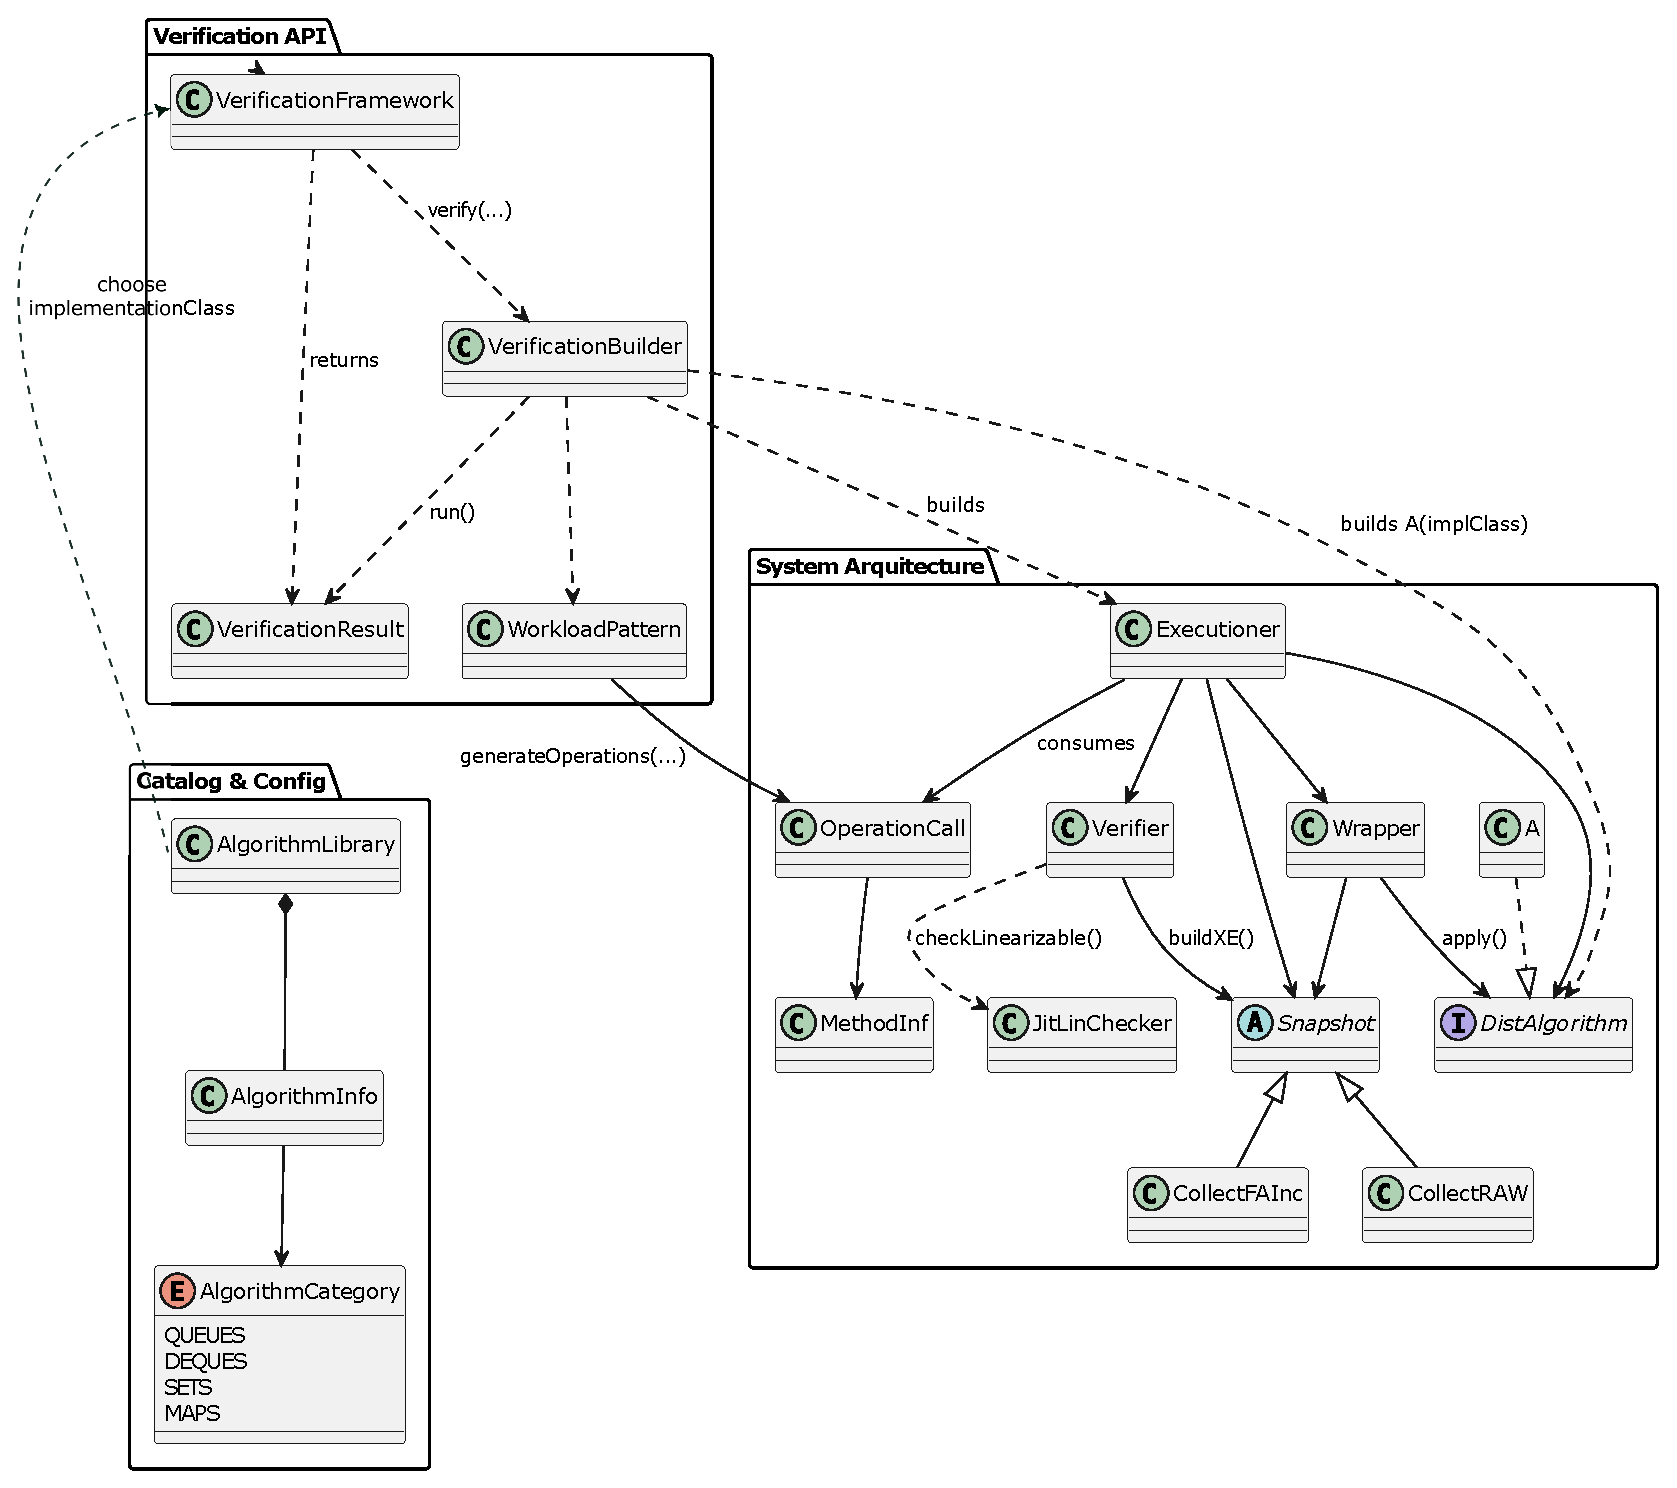
\includegraphics[width=\textwidth]{imgs/summary.eps}
    \caption{Interaction between the framework components during a verification run.}
    \label{fig:verificationFramework}
\end{figure}

At the highest level, a user selects a concurrent implementation via the
\texttt{VerificationFramework} API, which constructs an execution environment
and returns a \texttt{VerificationResult}. Internally, the framework is
organized in two layers: an \emph{instrumentation layer} responsible for
detecting the execution, and a \emph{monitoring layer} responsible for
deciding linearizability.

%─────────────────────────────────────────────────────────────────────────────
\subsection{Instrumentation Layer}
\label{subsec:instrumentation}
%─────────────────────────────────────────────────────────────────────────────

The instrumentation layer intercepts every operation invocation and response
without modifying the implementation under inspection. It consists of the
\texttt{Wrapper} and the \texttt{Snapshot} object.

The Wrapper (Algorithm~\ref{alg:wrapper}) is a concurrent algorithm where worker threads record invocation and response events for each operation. These events are written to a shared \texttt{Snapshot} object, following the protocol in~\cite{CR23}.

\begin{algorithm}[H]
\scriptsize
\caption{Wrapper: distributed instrumentation mechanism}
\label{alg:wrapper}
\begin{algorithmic}[1]
\Procedure{Execute}{$op, params$}
  \State $id \gets \textbf{ThreadId}()$
  \State $C.\textsc{Write}(id, \langle \textit{invoke}, op, params \rangle)$
  \State $res \gets A.\textsc{Apply}(op, params)$
  \State $C.\textsc{Snapshot}(id, \langle \textit{return}, res \rangle)$
\EndProcedure
\end{algorithmic}
\end{algorithm}

\paragraph{Snapshot objects.}
The framework provides two non-linearizable collect implementations that
share a common interface: \texttt{write}, \texttt{snapshot}, \texttt{buildXE} (Algorithms~\ref{alg:collectfainc} and~\ref{alg:collectraw}).
Both are implemented in Clojure.

% ─── CollectFAInc ───────────────────────────────────────────────────────────

\textsc{CollectFAInc} (identifier \texttt{gAIsnap} in the repository)
induces a total order on all events using a single shared atomic
fetch-and-increment counter. Every call to \texttt{write} or \texttt{snapshot}
atomically increments the counter and stores the resulting timestamp alongside
the event in the invoking thread's local log
(Algorithm~\ref{alg:collectfainc}). Because the counter is strictly monotone
and the increment is atomic, timestamps are globally unique and totally ordered
across threads. At the end of the execution, \texttt{buildXE} merges all
per-thread logs, sorts them by timestamp,
and returns the resulting sequence as $X_E$.

\begin{algorithm}[H]
\scriptsize
\caption{\textsc{CollectFAInc}: write and snapshot}
\label{alg:collectfainc}
\begin{algorithmic}[1]
\Procedure{Write}{$id, \langle invoke, op, params \rangle$}
  \State $cnt \gets \textbf{fetch-and-increment}(counter)$
  \State $opId \gets \langle id, localIndex[id]\mathtt{++} \rangle$
  \State $lastOpId[id] \gets opId$
  \State $log[id].\textbf{append}(\{$
      \texttt{:type}~$\mathbf{invoke},$
      \texttt{:op-id}~$opId,$
      \texttt{:tid}~$id,$
      \texttt{:op}~$op,$
      \texttt{:arg}~$params,$
      \texttt{:count}~$cnt\})$
\EndProcedure
\Procedure{Snapshot}{$id, \langle return, res \rangle$}
  \State $cnt \gets \textbf{fetch-and-increment}(counter)$
  \State $opId \gets lastOpId[id]$
  \State $log[id].\textbf{append}(\{$
      \texttt{:type}~$\mathbf{return},$
      \texttt{:op-id}~$opId,$
      \texttt{:tid}~$id,$
      \texttt{:res}~$res,$
      \texttt{:count}~$cnt\})$
\EndProcedure
\Procedure{BuildXE}{}
  \State $events \gets \bigcup_{i} log[i]$
  \State \Return $\textbf{sort}(events,\ \text{by}\ (\texttt{:count},\ \texttt{:tid}))$
\EndProcedure
\end{algorithmic}
\end{algorithm}

% ─── CollectRAW ─────────────────────────────────────────────────────────────

\textsc{CollectRAW} in Algorithm~\ref{alg:collectraw} 
(identifier \texttt{rawsnap} in the repository)
maintains two separate per-thread logs:
$\mathit{invs}[id]$ for invocations and $\mathit{rets}[id]$ for responses.
\textsc{Snapshot} reads the current invocation logs of
\emph{all} threads and stores this cross-thread view alongside the
response. \textsc{BuildXE} reconstructs the happens-before relation from
the captured views: if $opId_k$ appears in the view of $ret_i$, then
$inv_k$ started before $ret_i$ completed; if $view(i) \subsetneq view(j)$,
then $ret_i$ completed before $inv_j$ started. The resulting partial order
is obtained by a topological sort (Kahn's algorithm).


The invocation logs are read in \textsc{Snapshot} without additional
synchronization --- no \texttt{volatile} fields, no locks, no
\texttt{ConcurrentArrayList}. This is intentional and corresponds to the
theoretical model of a \emph{non-linearizable} collect object~\cite{RC24}:
the view captured at a response may miss invocations that are concurrently
being written. A partial view makes the observed execution \emph{more
concurrent} than the real one (fewer precedence edges are established),
never less. Soundness is preserved: if the observed execution --- with
potentially more concurrency --- is not linearizable, then the real
execution is also not linearizable.

\begin{algorithm}[H]
\scriptsize
\caption{\textsc{CollectRAW}: write, snapshot, and buildXE}
\label{alg:collectraw}
\begin{algorithmic}[1]
\Procedure{Write}{$id, \langle invoke, op, params \rangle$}
  \State $opId \gets \langle id, localIndex[id]\mathtt{++} \rangle$
  \State $lastOpId[id] \gets opId$
  \State $\mathit{invs}[id].\textbf{append}(\{$
      \texttt{:type}~$\mathbf{invoke},$
      \texttt{:op-id}~$opId,$
      \texttt{:tid}~$id,$
      \texttt{:op}~$op,$
      \texttt{:arg}~$params\})$
\EndProcedure
\Procedure{Snapshot}{$id, \langle return, res \rangle$}
  \State $view \gets \textbf{copy}(\mathit{invs}[0], \ldots, \mathit{invs}[n{-}1])$
      \Comment{snapshot of all invocations}
  \State $opId \gets lastOpId[id]$
  \State $\mathit{rets}[id].\textbf{append}(\{$
      \texttt{:type}~$\mathbf{return},$
      \texttt{:op-id}~$opId,$
      \texttt{:tid}~$id,$
      \texttt{:res}~$res,$
      \texttt{:view}~$view\})$
\EndProcedure
\Procedure{BuildXE}{}
  \State Build edges of a partial order:
  \State \quad (a) $inv_x \to ret_x$ for each complete operation $x$
  \State \quad (b) $ret_i \to inv_j$ if
      $\mathit{view}(i) \subsetneq \mathit{view}(j)$
      and $opId_j \notin \mathit{view}(i)$
      \Comment{$ret_i$ completed before $inv_j$ started}
  \State \quad (c) $inv_k \to ret_i$ if
      $opId_k \in \mathit{view}(i)$
      and $k \neq i$
      \Comment{$inv_k$ started before $ret_i$ completed}
  \State \Return $\textbf{topological-sort}(\text{edges})$
\EndProcedure
\end{algorithmic}
\end{algorithm}



%─────────────────────────────────────────────────────────────────────────────
\subsection{Monitoring Layer}
\label{subsec:monitoring}
%─────────────────────────────────────────────────────────────────────────────

After the instrumentation layer finishes collecting events, the monitoring
layer reconstructs a well-formed execution $X_E$ and decides its
linearizability.

The \texttt{Verifier} shares the \texttt{Snapshot} object with the
\texttt{Wrapper}. It calls \texttt{buildXE()} to obtain a well-formed execution
(\texttt{IPersistentVector}) of events and passes it to the
JIT-based linearizability checker (\texttt{JitLinChecker})~\cite{lowe2017}. 
If the observed execution
is \emph{not} linearizable, the framework guarantees that the real execution
is also not linearizable --- a soundness property inherited from the
non-linearizable collect objects~\cite{RC24}. The converse direction is not
guaranteed, which is unavoidable given the impossibility result
of~\cite{CR25_JACM}.

%─────────────────────────────────────────────────────────────────────────────
\subsection{Execution Environment}
\label{subsec:execution}
%─────────────────────────────────────────────────────────────────────────────

The \texttt{Executioner} instantiates the
\texttt{Snapshot}, \texttt{Wrapper}, and \texttt{Verifier} components, spawns
worker threads that invoke operations on the \texttt{DistAlgorithm} object,
and collects the final verdict and execution time.

\texttt{DistAlgorithm} is an abstraction layer for the concurrent
implementation under inspection. It wraps a Java concurrent class
via reflection, exposing a uniform \texttt{apply(method, args)} interface
that allows the framework to handle any data structure without modifying
its source code.

The \texttt{VerificationFramework} API (Figure~\ref{fig:verificationFramework})
exposes this execution environment to users through a builder pattern:
the user selects a concurrent class from the \texttt{AlgorithmLibrary}
(which catalogs queues, deques, sets, and maps), configures thread count
and snapshot strategy, and calls \texttt{run()} to obtain a
\texttt{VerificationResult}.

\section{Experimental Evaluation}
\label{sec:experiments}

We evaluate the framework along two axes: instrumentation overhead
and verdict accuracy. We follow the methodology of Georges
et al.~\cite{georges2007}: five warmup rounds (discarded) followed by
ten measured rounds per cell; we report mean execution time in
milliseconds. All experiments were run on a 64-core Linux server
(OpenJDK 21.0.10, \texttt{-Xmx16g}). The AspectJ variant uses
load-time weaving via \texttt{-javaagent:aspectjweaver}.
Figure~\ref{fig:benchmark} summarizes the main results.

%─────────────────────────────────────────────────────────────────
\subsection{Instrumentation Overhead}
%─────────────────────────────────────────────────────────────────

Tables~\ref{tab:ops} and~\ref{tab:threads} measure \texttt{taskProducers()}
time only --- no linearizability checking is performed. All experiments
use \texttt{\seqsplit{java.util.concurrent.ConcurrentLinkedQueue}} with operations
\texttt{offer} and \texttt{poll}.

\begin{table}[h!]
\centering
\scriptsize
\caption{Instrumentation overhead vs.\ operation count (mean ms,
         threads~=~4).}
\label{tab:ops}
\begin{tabular}{rrrr}
\hline
\textbf{Ops} & \texttt{CollectFAInc} & \texttt{CollectRAW} & AspectJ \\
\hline
       100 &     0 &     2 &     2 \\
       500 &     9 &     9 &     7 \\
     1\,000 &    20 &    21 &    16 \\
     5\,000 &   101 &   101 &    79 \\
    10\,000 &   204 &   204 &   160 \\
    50\,000 & 1\,031 & 1\,028 &   869 \\
   100\,000 & 2\,005 & 2\,002 & 1\,757 \\
\hline
\end{tabular}
\end{table}

\begin{table}[h!]
\centering
\scriptsize
\caption{Instrumentation overhead vs.\ thread count (mean ms,
         ops~=~10\,000).}
\label{tab:threads}
\begin{tabular}{rrrr}
\hline
\textbf{Threads} & \texttt{CollectFAInc} & \texttt{CollectRAW} & AspectJ \\
\hline
  2 &   160 &   159 &   133 \\
  4 &   204 &   204 &   160 \\
  8 &   373 &   379 &   250 \\
 16 &   476 &   482 &   378 \\
 32 &   560 &   563 &   439 \\
 64 &   608 &   593 &   507 \\
\hline
\end{tabular}
\end{table}

\texttt{CollectFAInc} and \texttt{CollectRAW} show virtually identical
overhead across all configurations (difference $<$1\% in all cells).
Both scale linearly with operation count: increasing ops by 10$\times$
yields approximately 10$\times$ more time (e.g., 20\,ms at 1\,000 ops
to 2\,005\,ms at 100\,000 ops with 4~threads). Scaling with thread count
is sub-linear: going from 2 to 64~threads (32$\times$) increases overhead
by approximately 4$\times$ at 10\,000 operations, indicating that the
framework distributes work effectively across cores.

AspectJ is consistently 20--30\% faster in raw instrumentation time
because \texttt{@AfterReturning} records a single event per operation
after completion, whereas the snapshot implementations record two events
(invocation and response) with shared-state access in between.
This performance gap does not reflect correctness, as shown next.

%─────────────────────────────────────────────────────────────────
\subsection{Verdict Accuracy on a Correct Implementation}
%─────────────────────────────────────────────────────────────────

Table~\ref{tab:verdicts} reports the percentage of correct verdicts
over 100 complete pipeline runs per cell (instrumentation + verification,
100~operations). Since \texttt{ConcurrentLinkedQueue} is a correct
implementation, the expected verdict is always \emph{linearizable}
(\%T~=~100, \%F~=~0, \%E~=~0).

\begin{table}[h!]
\centering
\scriptsize
\caption{Verdict accuracy over 100 runs (ops~=~100,
         \texttt{ConcurrentLinkedQueue}).
         \%T~=~linearizable, \%F~=~not linearizable, \%E~=~error.}
\label{tab:verdicts}
\begin{tabular}{rccccccccc}
\hline
\textbf{Thr.}
  & \multicolumn{3}{c}{\texttt{CollectFAInc}}
  & \multicolumn{3}{c}{\texttt{CollectRAW}}
  & \multicolumn{3}{c}{AspectJ} \\
  & \%T & \%F & \%E & \%T & \%F & \%E & \%T & \%F & \%E \\
\hline
 2 & 100 & 0 & 0 & 100 & 0 & 0 &  45 & 55 & 0 \\
 4 & 100 & 0 & 0 & 100 & 0 & 0 &  79 & 21 & 0 \\
 8 & 100 & 0 & 0 & 100 & 0 & 0 &  98 &  2 & 0 \\
16 & 100 & 0 & 0 & 100 & 0 & 0 &  99 &  1 & 0 \\
32 & 100 & 0 & 0 & 100 & 0 & 0 & 100 &  0 & 0 \\
64 & 100 & 0 & 0 & 100 & 0 & 0 & 100 &  0 & 0 \\
\hline
\end{tabular}
\end{table}

\texttt{CollectFAInc} and \texttt{CollectRAW} produce correct verdicts
in all 100 runs across all thread configurations. AspectJ produced false
negatives in 55\% of runs with 2~threads, decreasing monotonically to
0\% at 32 and 64~threads. This pattern reveals two regimes. Under
\emph{high CPU contention} (thread count $<$ available cores), threads
compete for CPU time and context switches between an operation's
completion and its trace capture in \texttt{@AfterReturning} are
frequent, producing observed executions that differ from the actual
order. Under \emph{genuine parallelism} (thread count $\geq$ cores),
each thread executes on a dedicated core without preemption, reducing the
non-atomicity window to near zero. This confirms the structural nature of
the observer effect identified by El-Hokayem and Falcone~\cite{E-HF18}.

\paragraph{Comparison with El-Hokayem and Falcone~\cite{E-HF18}.}
Their work identifies AspectJ bytecode weaving as the source of false
positives and false negatives in runtime verification, showing that the
observed execution may differ from the actual one due to the
non-atomicity of before/after instrumentation points. We use
\texttt{@AfterReturning} as a \emph{baseline instrumentation strategy},
isolating the instrumentation component from the verification component:
all three strategies use the same JIT-Lin checker~\cite{lowe2017}, so
any difference in verdict accuracy is attributable solely to
instrumentation. Their reference experiment reports false negative rates
of 92--99\% for AspectJ-based tools on an unsynchronized implementation.
Our results are complementary: using a \emph{correct} implementation,
AspectJ still produces false negatives (up to 55\%), while
\texttt{CollectFAInc} and \texttt{CollectRAW} produce 0\% in all
configurations.

A natural question is whether \texttt{@Around} advice --- which wraps
the entire operation in a single control block --- would close this
reliability gap. We leave a systematic comparison as future work; we
note, however, that \texttt{@Around} reduces but does not eliminate
the non-atomicity window, and provides no formal soundness guarantee
analogous to that of the collect objects~\cite{RC24}.

%─────────────────────────────────────────────────────────────────
\subsection{Verdict Accuracy on Non-Linearizable Implementations}
%─────────────────────────────────────────────────────────────────

\paragraph{Severely broken implementation.}
Table~\ref{tab:verdicts-broken} reports verdict accuracy for
\texttt{BrokenQueue}, an intentionally non-linearizable queue with a
severe race condition. The expected verdict is always \emph{not
linearizable} (\%T~=~0, \%F~=~100, \%E~=~0).

\begin{table}[h!]
\centering
\scriptsize
\caption{Verdict accuracy over 100 runs (ops~=~100, \texttt{BrokenQueue},
         expected: not linearizable).}
\label{tab:verdicts-broken}
\begin{tabular}{rccccccccc}
\hline
\textbf{Thr.}
  & \multicolumn{3}{c}{\texttt{CollectFAInc}}
  & \multicolumn{3}{c}{\texttt{CollectRAW}}
  & \multicolumn{3}{c}{AspectJ} \\
  & \%T & \%F & \%E & \%T & \%F & \%E & \%T & \%F & \%E \\
\hline
 2 & 0 & 100 & 0 & 0 & 100 & 0 & 0 & 100 & 0 \\
 4 & 0 & 100 & 0 & 0 & 100 & 0 & 0 & 100 & 0 \\
 8 & 0 & 100 & 0 & 0 & 100 & 0 & 0 & 100 & 0 \\
16 & 0 & 100 & 0 & 0 & 100 & 0 & 0 & 100 & 0 \\
32 & 0 & 100 & 0 & 0 & 100 & 0 & 0 & 100 & 0 \\
64 & 0 & 100 & 0 & 0 & 100 & 0 & 0 & 100 & 0 \\
\hline
\end{tabular}
\end{table}

All three strategies correctly identify \texttt{BrokenQueue} as
non-linearizable in 100\% of runs. The asymmetry with
Table~\ref{tab:verdicts} is the key finding: AspectJ-based
instrumentation produces false negatives exclusively on \emph{correct}
implementations --- precisely the scenario where unreliable verdicts
are most harmful, as a developer receiving a spurious non-linearizable
verdict may incorrectly modify code that does not need to change.

\paragraph{Subtly broken implementation.}
Table~\ref{tab:verdicts-partial} reports verdict accuracy for
\texttt{PartialSyncQueue}, an implementation with a subtle race
condition between \texttt{isEmpty()} and \texttt{removeFirst()} in
\texttt{poll()}: \texttt{offer()} is synchronized but \texttt{poll()}
is not, so a second thread may empty the queue between the
\texttt{isEmpty()} check and the \texttt{removeFirst()} call.
Unlike \texttt{BrokenQueue}, this violation manifests only under
specific interleavings and does not occur in every execution.

\begin{table}[h!]
\centering
\scriptsize
\caption{Verdict accuracy over 100 runs (ops~=~60,
         \texttt{PartialSyncQueue}).
         \%T~=~linearizable, \%F~=~not linearizable, \%E~=~error.}
\label{tab:verdicts-partial}
\begin{tabular}{rccccccccc}
\hline
\textbf{Thr.}
  & \multicolumn{3}{c}{\texttt{CollectFAInc}}
  & \multicolumn{3}{c}{\texttt{CollectRAW}}
  & \multicolumn{3}{c}{AspectJ} \\
  & \%T & \%F & \%E & \%T & \%F & \%E & \%T & \%F & \%E \\
\hline
 2 & 91 &  9 & 0 & 95 &  5 & 0 & 36 & 64 & 0 \\
 4 & 85 & 15 & 0 & 96 &  4 & 0 & 67 & 33 & 0 \\
 8 & 84 & 16 & 0 & 92 &  8 & 0 & 98 &  2 & 0 \\
16 & 97 &  3 & 0 & 94 &  6 & 0 &100 &  0 & 0 \\
32 &100 &  0 & 0 & 99 &  1 & 0 &100 &  0 & 0 \\
64 &100 &  0 & 0 & 99 &  1 & 0 &100 &  0 & 0 \\
\hline
\end{tabular}
\end{table}

The \%F column for \texttt{CollectFAInc} and \texttt{CollectRAW}
reflects the fraction of runs in which the race condition manifested
and was correctly detected (3--16\% depending on thread count). The
remaining runs correspond to executions where the violation did not
occur within 60 operations and the execution was genuinely
linearizable --- a correct verdict in both cases. No false positives
are produced: every non-linearizable verdict corresponds to a real
violation. AspectJ shows the opposite pattern at low thread counts:
with 2~threads, it produces 64\% false negatives --- runs where the
violation occurred but the non-atomic instrumentation failed to capture
it, causing the verifier to see a linearizable trace. The contrast
between Tables~\ref{tab:verdicts-broken} and~\ref{tab:verdicts-partial}
illustrates the key distinction between detection rate and soundness:
\texttt{CollectFAInc} and \texttt{CollectRAW} are sound in both cases,
whether the implementation is severely broken or only subtly so.

%─────────────────────────────────────────────────────────────────
\subsection{Coverage Across Data Structure Types}
%─────────────────────────────────────────────────────────────────

Table~\ref{tab:tableE} evaluates the framework across all supported
data structure types (threads~=~4, ops~=~30, 10~runs per cell) on the
64-core Linux server. Results were consistent with a separate run on a
10-core macOS laptop, confirming that the observed behavior is
independent of the hardware platform.

\begin{table}[h!]
\centering
\scriptsize
\caption{Coverage across data structure types (threads~=~4, ops~=~30,
         10~runs). OK~=~verdict matches expected;
         FAIL~=~unexpected verdict.}
\label{tab:tableE}
\begin{tabular}{llccccc}
\hline
\textbf{Implementation} & \textbf{Exp.}
  & \multicolumn{2}{c}{\texttt{CollectFAInc}}
  & \multicolumn{2}{c}{\texttt{CollectRAW}}
  & \textbf{AspectJ} \\
  & & \%T & Match & \%T & Match & Match \\
\hline
\multicolumn{7}{l}{\textit{Queues}} \\
ConcurrentLinkedQueue  & LIN & 100 & OK & 100 & OK & OK (60\%T) \\
LinkedBlockingQueue    & LIN & 100 & OK & 100 & OK & OK (70\%T) \\
LinkedTransferQueue    & LIN & 100 & OK & 100 & OK & OK (60\%T) \\
\multicolumn{7}{l}{\textit{Deques}} \\
ConcurrentLinkedDeque  & LIN & 100 & OK & 100 & OK & OK (60\%T) \\
LinkedBlockingDeque    & LIN & 100 & OK & 100 & OK & OK (90\%T) \\
\multicolumn{7}{l}{\textit{Sets}} \\
ConcurrentSkipListSet  & LIN & 100 & OK & 100 & OK & OK (100\%T) \\
\multicolumn{7}{l}{\textit{Maps}} \\
ConcurrentHashMap      & LIN & 100 & OK & 100 & OK & \textbf{FAIL (0\%T)} \\
ConcurrentSkipListMap  & LIN & 100 & OK & 100 & OK & \textbf{FAIL (0\%T)} \\
\multicolumn{7}{l}{\textit{Non-linearizable implementations}} \\
BrokenQueue            & NOT &   0 & OK &   0 & OK & OK (0\%T)  \\
NonLinearizableQueue   & NOT &  10 & OK &  10 & OK & OK (10\%T) \\
PartialSyncQueue       & NOT &  90 & OK &  95 & OK & OK (60\%T) \\
\hline
\end{tabular}
\end{table}

\texttt{CollectFAInc} and \texttt{CollectRAW} produce correct verdicts
for all 11 implementations. AspectJ produces false negatives in queue
and deque implementations (10--40\%) and fails entirely on map
implementations, reporting 100\% false negatives for both
\texttt{ConcurrentHashMap} and \texttt{ConcurrentSkipListMap}. This
failure on maps is consistent across both test machines and is
attributable to incorrect argument capture in \texttt{@AfterReturning}
for multi-argument operations such as \texttt{put(key,\,value)}: the
resulting trace is structurally malformed for the verifier,
independently of the thread scheduler.

%─────────────────────────────────────────────────────────────────
% Figura de resumen — generada con fig_benchmark.py
%─────────────────────────────────────────────────────────────────

\begin{figure}[t]
\centering
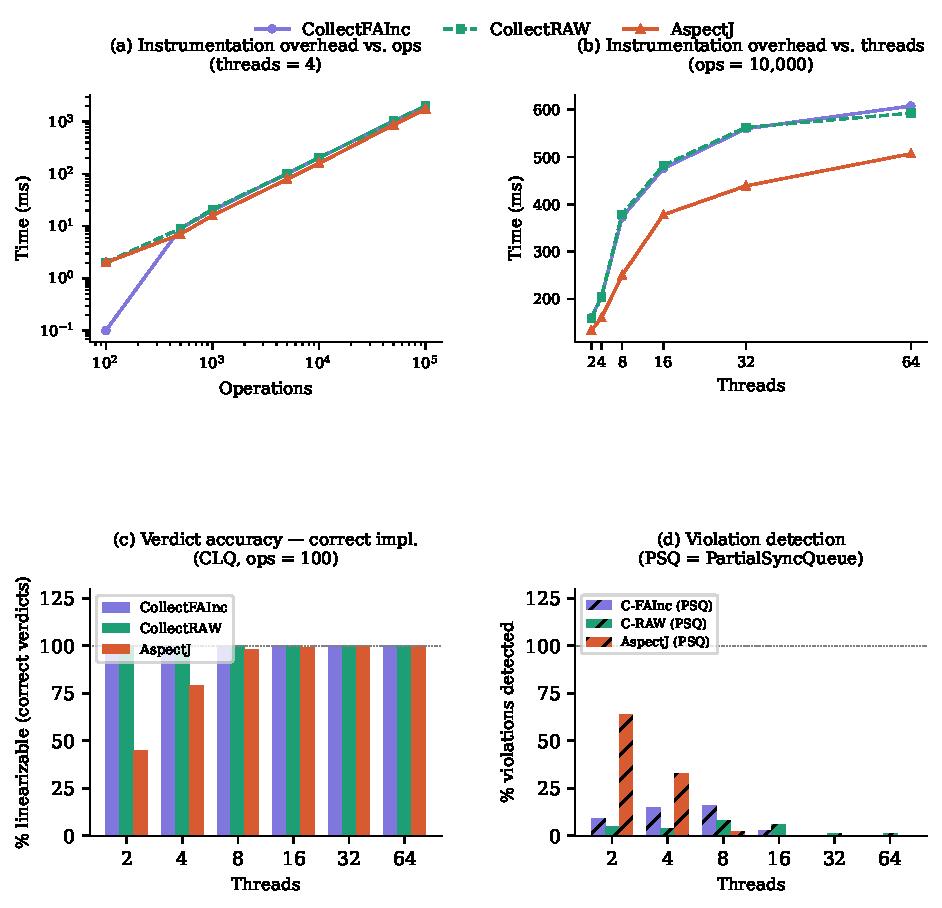
\includegraphics[width=\textwidth]{fig_benchmark.pdf}
\caption{Summary of experimental results.
  \textbf{(a)}~Instrumentation overhead vs.\ operation count (threads~=~4,
  log--log scale).
  \textbf{(b)}~Instrumentation overhead vs.\ thread count (ops~=~10\,000).
  \textbf{(c)}~Verdict accuracy on a correct implementation
  (\texttt{ConcurrentLinkedQueue}, ops~=~100, 100~runs per cell):
  \texttt{CollectFAInc} and \texttt{CollectRAW} achieve 100\% correct
  verdicts at all thread counts; AspectJ degrades to 45\% under
  contention.
  \textbf{(d)}~Violation detection rate for
  \texttt{BrokenQueue}~(BQ, severe race condition)
  and \texttt{PartialSyncQueue}~(PSQ, subtle race condition).
  All strategies detect BQ in 100\% of runs; PSQ detection varies
  with the manifestation rate of the race condition.}
\label{fig:benchmark}
\end{figure}

\paragraph{Note on sample size.}
Due to the NP-completeness of linearizability checking~\cite{GK97},
verdict experiments are limited to 60--100~operations and 100~runs per
cell, except Table~\ref{tab:tableE} which uses 10~runs per cell.
The observed trends are consistent with the theoretical predictions
of~\cite{E-HF18}.


\section{Usage and Availability}

The framework is implemented in Java and Clojure, built with Maven,
and distributed under the Apache~2.0 license at:
\begin{center}
\url{https://github.com/PRISM-Concurrent/efficient-distributed-rv}
\end{center}

\paragraph{Minimal usage example.}
To verify a \texttt{ConcurrentLinkedQueue} with 4 threads and
100 operations, a user writes:

\begin{verbatim}
VerificationResult result = VerificationFramework
    .forClass("java.util.concurrent.ConcurrentLinkedQueue")
    .withThreads(4)
    .withOperations(100)
    .withSnapshot("CollectFAInc")
    .verify();
System.out.println(result.isLinearizable());
\end{verbatim}

No modifications to the implementation under test are required.
The framework can be extended to other data structures by providing
a sequential specification in Clojure following the examples in
\texttt{src/main/clojure/spec/}.

\paragraph{Reproducing the experiments.}
The results reported in Tables~\ref{tab:ops}--\ref{tab:verdicts}
can be reproduced with:

\begin{verbatim}
mvn clean package -DskipTests
java -cp target/efficient-distributed-rv-*-jar-with-dependencies.jar \
     phd.experiments.VerifierBenchmark --format=org \
     --output=results/verifier.org
\end{verbatim}

The repository includes detailed documentation
(\texttt{README.md}, \texttt{QUICK\_START.md}),
example workloads, and configuration files.

\section{Related Work}
\label{sec:related}

Several tools perform runtime verification for concurrent Java programs using
intrusive instrumentation. Java-MOP~\cite{CR05}, Tracematches~\cite{BHL10},
and LARVA~\cite{CPS09} generate monitors from formal specifications and rely
on AspectJ for instrumentation. As shown experimentally by El-Hokayem and
Falcone~\cite{E-HF18}, this approach introduces false positives and false
negatives because the observed execution may differ from the actual one ---
a problem our framework avoids by design. These tools also focus on
sequential properties expressed in total-order formalisms (LTL, FSMs, regular
expressions), whereas linearizability is inherently a property of partial
orders.

Tools such as JPaX~\cite{HR04} and RVPredict~\cite{HMR14} target specific
concurrency errors --- data race freedom and deadlock freedom --- rather than
linearizability. Their underlying models (lockset analysis, maximal causal
models) are well-suited to those properties but do not generalize to
linearizability checking.

The closest related work on the verification side is the JIT-based
linearizability checker of Lowe~\cite{lowe2017}, which our framework
integrates in the monitoring layer. Lowe's tool addresses the decision
problem but assumes the execution has already been correctly captured; it
does not address the instrumentation problem. Our framework complements
this checker with a non-intrusive instrumentation layer that provides the
soundness guarantee absent from AspectJ-based approaches.

%\section{Acknowledgments}

%Gilde Valeria Rodríguez is the recipient of a PhD fellowship
%from SECIHTI.
%Armando Castañeda is supported by the research
%projects DGAPA-PAPIIT IN108723 and IN103126, and SECIHTI CBF-2025-I-393.

\section*{Software Metadata}

\begin{table}[H]
\centering
\small
\begin{tabular}{p{0.30\textwidth} p{0.65\textwidth}}
\hline
\textbf{Item} & \textbf{Description} \\
\hline
Software name & Distributed Runtime Verification Framework of Linearizability\\
Version & v1.0.0 \\
Release date & 2025-12-15 \\
%//Authors & Gilde Valeria Rodríguez; Miguel Piña; Armando Castañeda \\
Authors & Anonymous (to be filled after review) \\
Repository (public) & \url{https://github.com/PRISM-Concurrent/efficient-distributed-rv} \\
Persistent identifier (DOI) & To be assigned \\
License & Apache License, Version 2.0 (Apache-2.0) \\
Programming language & Java, Clojure \\
Build system & Maven \\
Operating systems & Linux, macOS, Windows \\
Requirements & JDK 21+, Maven 3.9+, Clojure runtime \\
Documentation & \texttt{README.md}, \texttt{INSTALL.md}, \texttt{API\_USAGE\_GUIDE.org}, \texttt{USER\_MANUAL.md}, \texttt{API\_EXAMPLES.md}, \texttt{QUICK\_START.md} \\
Support email & Available after acceptance \\ %miguelpinia1@gmail.com, gildevroji@gmail.com \\
\hline
\end{tabular}
\caption{Software metadata required for an Original Software Publication.}
\label{tab:software-metadata}
\end{table}

\paragraph{Declaration of generative AI and AI-assisted technologies in the manuscript
preparation process} 
During the preparation of this work, the authors used
Claude in order to assist with language editing, grammar, style revision,
and \LaTeX formatting of the manuscript. After using this tool, the authors
reviewed and edited the content as needed and take full responsibility for the
content of the published article.


\paragraph{Declaration of interests} 
The authors declare that they have 
no known competing financial interests or 
personal relationships that could have appeared to 
influence the work reported in this paper.

% (Content to be added)
\bibliographystyle{elsarticle-harv}
\bibliography{biblio}

\end{document}

%%% Local Variables:
%%% mode: LaTeX
%%% TeX-master: t
%%% End:
